\documentclass[../EDI_Task4_Karwowski_Kowalewski.tex]{subfiles}

\begin{document} {

    Zbiorem treningowym były obrazy \textit{03.bmp} oraz \textit{06.bmp}.
    \begin{figure}[!htbp]
        \begin{minipage}[c]{0.49\linewidth}
            \centering
            \includegraphics[width=0.75\textwidth]{img/results_3/4/compressed_08.png}
            \caption{Liczba neuronów 4}
        \end{minipage}\hfill
        \begin{minipage}[c]{0.49\linewidth}
            \centering
            \includegraphics[width=0.75\textwidth]{img/results_3/8/compressed_08.png}
            \caption{Liczba neuronów 8}
        \end{minipage}
    \end{figure}

    \begin{figure}[!htbp]
        \begin{minipage}[c]{0.49\linewidth}
            \centering
            \includegraphics[width=0.75\textwidth]{img/results_3/16/compressed_08.png}
            \caption{Liczba neuronów 16}
        \end{minipage}\hfill
        \begin{minipage}[c]{0.49\linewidth}
            \centering
            \includegraphics[width=0.75\textwidth]{img/results_3/32/compressed_08.png}
            \caption{Liczba neuronów 32}
        \end{minipage}
    \end{figure}

    \begin{figure}[!htbp]
        \centering
        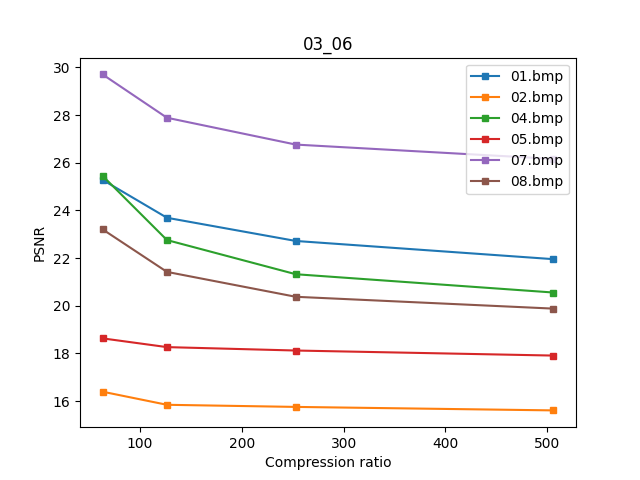
\includegraphics[width=0.75\textwidth]{img/results_3/stats_03_06.png}
        \caption{Wykres stopnia kompresji od PSNR}
    \end{figure}
    \FloatBarrier
}
\end{document}
